% questions.tex —— 2006 年·普通高等学校招生考试·浙江卷理科 · 题目内容片段（无答案）
% 由 tools/generate_projects.py 依来源总账自 2006/2006_数学真题_浙江理_试题.md 生成，勿手改（改源 MD 后重跑）


\begin{gktip}
\textbf{来源及状态}：据固定 PDF 第 1–2 页逐题目视转录；固定文件 SHA-256 与指定 Source ID 所登记的摘要一致。首页可见题签为“2006 普通高等学校招生考试（浙江卷理）”。题签和文件字节指纹只描述本次固定副本及页内可见文字，不能认证发布者、出版版次、来源链或官方原件身份。本稿不补答案、解析或评分信息。

\textbf{源页定位}：PDF 第 1 页（印刷页码 340）含 Q1–Q17；第 2 页（印刷页码 341）含 Q18–Q20。选择题 Q1–Q10，填空题 Q11–Q14，解答题 Q15–Q20。源页未标逐题分值或总分。

\textbf{题图}：Q9、Q14、Q15、Q17、Q19、Q20 已按固定候选 PDF 对照重绘为 TikZ 矢量图；未标尺寸的空间关系仅作示意。Q15 参数范围按源页保留为闭区间。题图仍需随正式项目版面复核。
\end{gktip}

\gkpart{一、选择题}

\begin{question}
\gkti{1}设集合 $A=\{x\mid -1\leqslant x\leqslant2\}$，$B=\{x\mid 0\leqslant x\leqslant4\}$，则 $A\cap B=$\mbox{（　　）}

（A）$[0,2]$　（B）$[1,2]$　（C）$[0,4]$　（D）$[1,4]$

\end{question}
\begin{question}
\gkti{2}已知 $\dfrac{m}{1+i}=1-ni$，其中 $m,n$ 是实数，$i$ 是虚数单位，则 $m+ni=$\mbox{（　　）}

（A）$1+2i$　（B）$1-2i$　（C）$2+i$　（D）$2-i$

\end{question}
\begin{question}
\gkti{3}已知 $0<a<1$，$\log_a m<\log_a n<0$，则\mbox{（　　）}

（A）$1<n<m$　（B）$1<m<n$　（C）$m<n<1$　（D）$n<m<1$

\end{question}
\begin{question}
\gkti{4}在平面直角坐标系中，不等式组
\nopagebreak[4]
\[
\begin{cases}
x+y-2\geqslant0,\\
x-y+2\geqslant0,\\
x\leqslant2
\end{cases}
\]
表示的平面区域的面积是\mbox{（　　）}

（A）$4\sqrt2$　（B）$4$　（C）$2\sqrt2$　（D）$2$

\end{question}
\begin{question}
\gkti{5}若双曲线 $\dfrac{x^2}{m}-y^2=1$ 上的点到左准线的距离是到左焦点距离的 $\dfrac13$，则 $m=$\mbox{（　　）}

（A）$\dfrac12$　（B）$\dfrac32$　（C）$\dfrac18$　（D）$\dfrac98$

\end{question}
\begin{question}
\gkti{6}函数 $y=\dfrac12\sin2x+\sin^2x$，$x\in\mathbb R$ 的值域是\mbox{（　　）}

（A）$\left[-\dfrac12,\dfrac32\right]$　（B）$\left[-\dfrac32,\dfrac12\right]$

（C）$\left[-\dfrac{\sqrt2}{2}+\dfrac12,\dfrac{\sqrt2}{2}+\dfrac12\right]$　（D）$\left[-\dfrac{\sqrt2}{2}-\dfrac12,\dfrac{\sqrt2}{2}-\dfrac12\right]$

\end{question}
\begin{question}
\gkti{7}“$a>b>0$”是“$ab<\dfrac{a^2+b^2}{2}$”的\mbox{（　　）}

（A）充分而不必要条件　（B）必要而不充分条件

（C）充分必要条件　（D）既不充分也不必要条件

\end{question}
\begin{question}
\gkti{8}若多项式 $x^2+x^{10}=a_0+a_1(x+1)+\cdots+a_9(x+1)^9+a_{10}(x+1)^{10}$，则 $a_9=$\mbox{（　　）}

（A）$9$　（B）$10$　（C）$-9$　（D）$-10$

\Needspace{0.4\textheight}
\end{question}
\begin{question}
\gkti{9}如图，$O$ 是半径为 $1$ 的球心，点 $A,B,C$ 在球面上，$OA,OB,OC$ 两两垂直，$E,F$ 分别是大圆弧 $\widehat{AB}$ 与 $\widehat{AC}$ 的中点，则点 $E,F$ 在该球面上的球面距离是\mbox{（　　）}

（A）$\dfrac{\pi}{4}$　（B）$\dfrac{\pi}{3}$　（C）$\dfrac{\pi}{2}$　（D）$\dfrac{\sqrt2\pi}{4}$
\nopagebreak[4]
\begin{center}% Source: fixed 2006 Zhejiang science scan, PDF page 1, Q9.
% Schematic projection; retain the three mutually perpendicular radii and
% the arc-midpoint labels on the great-circle arcs AB and AC.
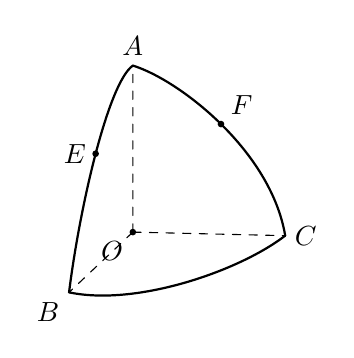
\begin{tikzpicture}[line cap=round,line join=round,x=0.9cm,y=0.9cm]
  \coordinate (O) at (0,0);
  \coordinate (A) at (0,2.35);
  \coordinate (B) at (-0.9,-0.85);
  \coordinate (C) at (2.15,-0.05);
  % Parameter midpoints of the two schematic cubic Bezier arcs.
  \coordinate (E) at (-0.525,1.10625);
  \coordinate (F) at (1.24375,1.525);
  % Schematic visible spherical boundary and the two great-circle arcs.
  \draw[thick] (A) .. controls (-0.35,2.1) and (-0.75,0.35) .. (B);
  \draw[thick] (A) .. controls (0.65,2.15) and (1.95,1.15) .. (C);
  \draw[thick] (B) .. controls (0.05,-1.05) and (1.5,-0.55) .. (C);
  \draw[dashed] (O)--(A) (O)--(B) (O)--(C);
  \fill (O) circle (1.2pt) (E) circle (1.2pt) (F) circle (1.2pt);
  \node[above] at (A) {$A$};
  \node[below left] at (B) {$B$};
  \node[right] at (C) {$C$};
  \node[below left] at (O) {$O$};
  \node[left] at (E) {$E$};
  \node[above right] at (F) {$F$};
\end{tikzpicture}
\end{center}
\nopagebreak[4]
\end{question}
\begin{question}
\gkti{10}函数 $f:\{1,2,3\}\to\{1,2,3\}$ 满足 $f(f(x))=f(x)$，则这样的函数个数共有\mbox{（　　）}

（A）$1$ 个　（B）$4$ 个　（C）$8$ 个　（D）$10$ 个

\end{question}
\gkpart{二、填空题}

\begin{question}
\gkti{11}设 $S_n$ 为等差数列 $\{a_n\}$ 的前 $n$ 项和，若 $S_5=10$，$S_{10}=-5$，则公差为 \gkblank{}。（用数字作答）

\end{question}
\begin{question}
\gkti{12}对 $a,b\in\mathbb R$，记
\nopagebreak[4]
\[
\max\{a,b\}=\begin{cases}
a,&a\geqslant b,\\
b,&a<b,
\end{cases}
\]
函数 $f(x)=\max\{|x+1|,|x-2|\}$（$x\in\mathbb R$）的最小值是 \gkblank{}。

\end{question}
\begin{question}
\gkti{13}设向量 $\boldsymbol a,\boldsymbol b,\boldsymbol c$ 满足 $\boldsymbol a+\boldsymbol b+\boldsymbol c=\boldsymbol0$，$(\boldsymbol a-\boldsymbol b)\perp\boldsymbol c$，$\boldsymbol a\perp\boldsymbol b$，若 $|\boldsymbol a|=1$，则 $|\boldsymbol a|^2+|\boldsymbol b|^2+|\boldsymbol c|^2$ 的值是 \gkblank{}。

\Needspace{0.4\textheight}
\end{question}
\begin{question}
\gkti{14}正四面体 $ABCD$ 的棱长为 $1$，棱 $AB$ 平行于平面 $\alpha$，则正四面体上的所有点在平面 $\alpha$ 内的射影构成的图形面积的取值范围是 \gkblank{}。
\nopagebreak[4]
\begin{center}% Source: fixed 2006 Zhejiang science scan, PDF page 1, Q14.
% Schematic projection; solid and hidden tetrahedron edges follow the scan.
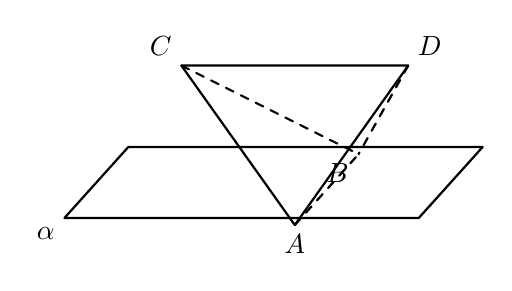
\begin{tikzpicture}[line cap=round,line join=round,x=0.9cm,y=0.9cm]
  \coordinate (C) at (0,2.5);
  \coordinate (D) at (3.2,2.5);
  \coordinate (A) at (1.6,0.25);
  % AB is parallel to the slanted side direction of the alpha plane.
  \coordinate (B) at (2.5,1.25);
  \coordinate (L) at (-0.75,1.35);
  \coordinate (R) at (4.25,1.35);
  \coordinate (Lb) at (-1.65,0.35);
  \coordinate (Rb) at (3.35,0.35);
  \draw[thick] (L)--(R)--(Rb)--(Lb)--cycle;
  \draw[thick] (C)--(D) (C)--(A) (D)--(A);
  \draw[thick,dashed] (C)--(B) (D)--(B) (A)--(B);
  \node[above left] at (C) {$C$};
  \node[above right] at (D) {$D$};
  \node[below] at (A) {$A$};
  \node[below left] at (B) {$B$};
  \node[below left] at (Lb) {$\alpha$};
\end{tikzpicture}
\end{center}
\nopagebreak[4]
\end{question}
\gkpart{三、解答题}

\Needspace{0.4\textheight}
\begin{question}
\gkti{15}如图，函数 $y=2\sin(\pi x+\varphi)$，$x\in\mathbb R$（其中 $0\leqslant\varphi\leqslant\dfrac{\pi}{2}$）的图象与 $y$ 轴交于点 $(0,1)$。

（1） 求 $\varphi$ 的值；

（2） 设 $P$ 是图象上的最高点，$M,N$ 是图象与 $x$ 轴的交点，求 $\overrightarrow{PM}$ 与 $\overrightarrow{PN}$ 的夹角。
\nopagebreak[4]
\begin{center}% Source: fixed 2006 Zhejiang science scan, PDF page 1, Q15.
% The plotted phase is schematic but respects the transcribed closed range
% 0 <= phi <= pi/2; M and N are adjacent x-intercepts around peak P.
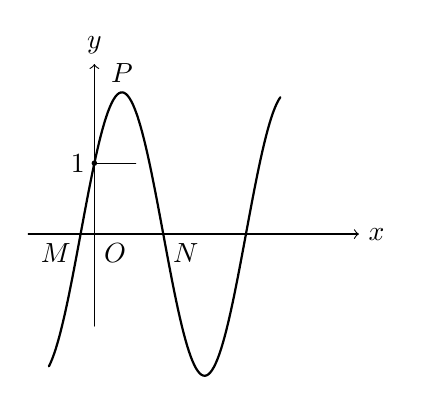
\begin{tikzpicture}[line cap=round,line join=round,x=1.05cm,y=0.9cm]
  \draw[->] (-0.8,0)--(3.2,0) node[right] {$x$};
  \draw[->] (0,-1.3)--(0,2.4) node[above] {$y$};
  \draw[thick] plot[domain=-0.55:2.25,samples=130] (\x,{2*sin(180*\x+30)});
  \draw (0,1)--(0.5,1);
  \node[left] at (0,1) {$1$};
  \fill (0,1) circle (1pt);
  \node[above] at (1/3,2) {$P$};
  \node[below left] at (-1/6,0) {$M$};
  \node[below right] at (5/6,0) {$N$};
  \node[below right] at (0,0) {$O$};
\end{tikzpicture}
\end{center}
\nopagebreak[4]
\end{question}
\begin{question}
\gkti{16}设 $f(x)=3ax^2+2bx+c$。若 $a+b+c=0$，$f(0)>0$，$f(1)>0$，求证：

（1） $a>0$ 且 $-2<\dfrac ba<-1$；

（2） 方程 $f(x)=0$ 在 $(0,1)$ 内有两个实根。

\Needspace{0.4\textheight}
\end{question}
\begin{question}
\gkti{17}如图，在四棱锥 $P-ABCD$ 中，底面为直角梯形，$AD\parallel BC$，$\angle BAD=90^\circ$，$PA\perp$ 底面 $ABCD$，且 $PA=AD=AB=2BC$，$M,N$ 分别为 $PC,PB$ 的中点。

（1） 求证：$PB\perp DM$；

（2） 求 $CD$ 与平面 $ADMN$ 所成的角。
\nopagebreak[4]
\begin{center}% Source: fixed 2006 Zhejiang science scan, PDF page 1, Q17.
% Schematic oblique projection; labels and solid/hidden edge relations follow
% the printed figure. M and N lie on PC and PB respectively.
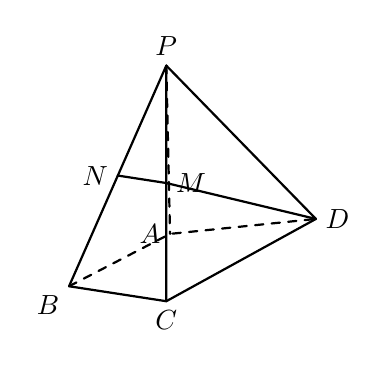
\begin{tikzpicture}[line cap=round,line join=round,x=0.95cm,y=0.95cm]
  \coordinate (P) at (1.55,3.1);
  \coordinate (A) at (1.6,0.85);
  \coordinate (B) at (0.25,0.15);
  \coordinate (C) at (1.55,-0.05);
  \coordinate (D) at (3.55,1.05);
  \coordinate (N) at (0.9,1.63);
  \coordinate (M) at (1.55,1.53);
  \draw[thick] (P)--(B)--(C)--(D)--cycle;
  \draw[thick] (P)--(C) (N)--(M)--(D);
  \draw[thick,dashed] (P)--(A) (B)--(A)--(D);
  \node[above] at (P) {$P$};
  \node[left] at (A) {$A$};
  \node[below left] at (B) {$B$};
  \node[below] at (C) {$C$};
  \node[right] at (D) {$D$};
  \node[left] at (N) {$N$};
  \node[right] at (M) {$M$};
\end{tikzpicture}
\end{center}
\nopagebreak[4]
\end{question}
\begin{question}
\gkti{18}甲、乙两袋装有大小相同的红球和白球，甲袋装有 $2$ 个红球、$2$ 个白球，乙袋装有 $2$ 个红球、$n$ 个白球。现从甲、乙两袋中各任取 $2$ 个球。

（1） 若 $n=3$，求取到的 $4$ 个球全是红球的概率；

（2） 若取到的 $4$ 个球中至少有 $2$ 个红球的概率为 $\dfrac34$，求 $n$。

\Needspace{0.4\textheight}
\end{question}
\begin{question}
\gkti{19}如图，椭圆 $\dfrac{x^2}{a^2}+\dfrac{y^2}{b^2}=1$（$a>b>0$）与过点 $A(2,0),B(0,1)$ 的直线有且只有一个公共点 $T$，且椭圆的离心率 $e=\dfrac{\sqrt3}{2}$。

（1） 求椭圆方程；

（2） 设 $F_1,F_2$ 分别为椭圆的左、右焦点，$M$ 为线段 $AF_2$ 的中点，求证：$\angle ATM=\angle AF_1T$。
\nopagebreak[4]
\begin{center}% Source: fixed 2006 Zhejiang science scan, PDF page 2, Q19.
% Schematic coordinate drawing; retain ellipse, foci, A/B, tangent point T,
% and the midpoint M of AF_2 with the labelled line segments shown in the scan.
\begin{tikzpicture}[line cap=round,line join=round,x=1.05cm,y=1.05cm]
  \draw[->] (-3.8,0)--(4.2,0) node[right] {$x$};
  \draw[->] (0,-2.25)--(0,2.35) node[above] {$y$};
  % Coordinates follow the stem: a^2=2, b^2=1/2, and c=sqrt(3/2).
  % The tangent AB touches at T=(1,1/2), and M is midpoint of AF_2.
  \draw[thick] (0,0) ellipse (1.41421 and 0.70711);
  \coordinate (A) at (2,0);
  \coordinate (B) at (0,1);
  \coordinate (T) at (1,0.5);
  \coordinate (Fone) at (-1.224745,0);
  \coordinate (Ftwo) at (1.224745,0);
  \coordinate (M) at (1.6123725,0);
  \draw[thick] (B)--(A);
  \draw (Fone)--(T) (T)--(M);
  \fill (Fone) circle (1.3pt) (Ftwo) circle (1.3pt);
  \node[above left] at (B) {$B$};
  \node[above right] at (T) {$T$};
  \node[below] at (A) {$A$};
  \node[below left] at (Fone) {$F_1$};
  \node[below right] at (Ftwo) {$F_2$};
  \node[below right] at (M) {$M$};
  \node[below left] at (0,0) {$O$};
\end{tikzpicture}
\end{center}
\nopagebreak[4]
\Needspace{0.4\textheight}
\end{question}
\begin{question}
\gkti{20}已知函数 $f(x)=x^3+x^2$，数列 $\{x_n\}$（$x_n>0$）的第一项 $x_1=1$，以后各项按如下方式取定：曲线 $y=f(x)$ 在 $(x_{n+1},f(x_{n+1}))$ 处的切线与经过 $(0,0)$ 和 $(x_n,f(x_n))$ 两点的直线平行（如图）。求证：当 $n\in\mathbb N^*$ 时，

（1） $x_n^2+x_n=3x_{n+1}^2+2x_{n+1}$；

（2） $\left(\dfrac12\right)^{n-1}\leqslant x_n\leqslant\left(\dfrac12\right)^{n-2}$。
\nopagebreak[4]
\begin{center}% Source: fixed 2006 Zhejiang science scan, PDF page 2, Q20.
% Schematic graph of y=x^3+x^2 with a secant from O to x_n and a parallel
% tangent at x_{n+1}; vertical guides identify both abscissae.
\begin{tikzpicture}[line cap=round,line join=round,x=1.15cm,y=0.8cm]
  \draw[->] (-0.8,0)--(3.5,0) node[right] {$x$};
  \draw[->] (0,-0.7)--(0,4.9) node[above] {$y$};
  \draw[thick] plot[domain=0:1.62,samples=100] (\x,{\x^3+\x^2});
  % s=0.6 and t=(-1+sqrt(10.12))/2 make f(t)/t=f'(s)=2.28.
  \coordinate (Q) at (0.6,0.576);
  \coordinate (R) at (1.090597372,2.486562008);
  \draw (0,0)--(R);
  \draw (0.18,-0.3816)--(1.02,1.5336);
  \draw[dashed] (0.6,0)--(Q) (1.090597372,0)--(R);
  \node[below left] at (0,0) {$O$};
  \node[below] at (0.6,0) {$x_{n+1}$};
  \node[below] at (1.090597372,0) {$x_n$};
\end{tikzpicture}
\end{center}
\nopagebreak[4]

\end{question}